% ============================================================
%  EAI 6020 – Module 3: Explainable AI Solution
%  APA 7 Professional Format | John Kingsley Arthur
% ============================================================
\documentclass[12pt,letterpaper]{article}

\usepackage[margin=1in]{geometry}
\usepackage{times}
\usepackage{setspace}
\usepackage{titlesec}
\usepackage{indentfirst}
\usepackage{fancyhdr}
% Allow URLs to break at hyphens (must precede hyperref/url load)
\PassOptionsToPackage{hyphens}{url}
\usepackage{hyperref}
\usepackage{url}
\usepackage{amsmath}
\usepackage{microtype}
\usepackage{graphicx}
\usepackage{booktabs}
\usepackage{caption}
\usepackage{float}
\usepackage[T1]{fontenc}
\usepackage[utf8]{inputenc}

% Graphics path – all PNG figures live in the same folder
\graphicspath{{./}}

% APA-style figure caption format
\captionsetup{font=singlespacing, labelfont=bf, labelsep=period,
              justification=raggedright, singlelinecheck=false}

% Allow URLs to break at any character to prevent margin overflow
% (PassOptionsToPackage moved before hyperref — see preamble top)

\doublespacing
\setlength{\parindent}{0.5in}
\setlength{\parskip}{0pt}
\setlength{\headheight}{15pt}

\pagestyle{fancy}
\fancyhf{}
\renewcommand{\headrulewidth}{0pt}
\rhead{\small EXPLAINABLE AI WITH VERTEX AI \quad \thepage}

\titleformat{\section}[block]{\normalfont\bfseries}{\thesection.}{0.5em}{}
\titlespacing*{\section}{0pt}{12pt}{6pt}
\titleformat{\subsection}[block]{\normalfont\bfseries\itshape}{\thesubsection}{0.5em}{}
\titlespacing*{\subsection}{0pt}{10pt}{4pt}

\hypersetup{colorlinks=false, breaklinks=true}

\begin{document}

% ============================================================
%  TITLE PAGE
% ============================================================
\thispagestyle{empty}
\begin{center}

\vspace*{1.2in}

Northeastern University\\[4pt]
EAI 6020 AI System Technologies

\vspace{0.55in}
\noindent\rule{0.65\textwidth}{0.4pt}
\vspace{0.35in}

{\large\bfseries Explainable AI with Vertex AI:}\\[10pt]
{\large\bfseries Platform Assessment, Model Evaluation,}\\[10pt]
{\large\bfseries and Feature Attribution Solutions}

\vspace{0.35in}
\noindent\rule{0.65\textwidth}{0.4pt}
\vspace{0.5in}

Module 3 Written Assignment

\vspace{0.55in}

\renewcommand{\arraystretch}{1.5}
\begin{tabular}{r l}
  \textbf{Student Name:} & JOHN KINGSLEY ARTHUR \\
  \textbf{Student ID:}   & 002301967 \\
  \textbf{Instructor:}   & Dr.\ Sohrob Milani Zadeh \\
  \textbf{Date:}         & June 5, 2026 \\
\end{tabular}

\end{center}
\newpage

% ============================================================
%  ABSTRACT
% ============================================================
\thispagestyle{fancy}
\noindent\textbf{Abstract}

Explainable artificial intelligence (XAI) has emerged as a critical component
of responsible AI deployment, enabling stakeholders to understand, audit, and
trust machine learning model decisions. This paper examines a hands-on
exploration of XAI capabilities using Google Cloud's Vertex AI platform, now
integrated into the Gemini Enterprise Agent Platform. The discussion covers the
rationale for selecting Vertex AI as the AI platform of choice, the
identification of appropriate predictive model evaluation metrics for a binary
classification task, and the development and experimentation with feature-based
explanations using Integrated Gradients and Sampled Shapley (SHAP). Empirical
observations from varying the number of approximation steps and paths, along
with the resulting impacts on attribution fidelity and computational cost, are
presented. The paper concludes with reflections on lessons learned and
implications for future ML pipeline design.

\vspace{6pt}
\noindent\textit{Keywords:} explainable AI, Vertex AI, feature attribution,
integrated gradients, model interpretability

\section{Introduction}

The rapid adoption of machine learning (ML) across high-stakes domains---including
healthcare, finance, and criminal justice---has intensified demands for model
transparency and accountability. As Lipton (2018) notes, interpretability in ML
is not a singular concept but a multidimensional property that encompasses
simulatability, decomposability, and algorithmic transparency. The field of
Explainable AI (XAI) addresses these concerns by providing human-understandable
explanations for model predictions, helping practitioners identify bias, validate
model behavior, and build trust with end-users (Doshi-Velez \& Kim, 2017). As
Philip (2019) observes, XAI can adopt either model-agnostic approaches---treating
the model as a black box---or model-specific approaches that exploit the internal
structure of a known algorithm; each carries distinct tradeoffs in scope,
computational cost, and explanatory fidelity.

This paper documents a hands-on exploration of XAI principles through Google
Cloud's Vertex AI platform. The primary objective was to implement feature
attribution explanations for a binary classification model, experiment with key
XAI configuration parameters---specifically the number of integral approximation
steps and the number of paths---and assess the resulting tradeoffs. The exercise
followed the ``Getting Explanations Locally in Notebook'' workflow and the Vertex
Pipelines framework for MLOps orchestration (Google Cloud, 2026a; Google Cloud,
2026b).

\section{AI Platform Service Selection and Assessment}

Several enterprise AI platforms were considered for this exercise, including
Microsoft Azure Machine Learning, Amazon SageMaker, and Google Cloud Vertex AI.
Azure ML offers strong integration with the Microsoft ecosystem but requires
additional configuration to access interpretability tooling at the depth provided
natively by Vertex AI. SageMaker Clarify provides bias and explainability
reporting, yet its feature attribution methods are less tightly integrated with
pipeline orchestration than Vertex AI Pipelines. Google Cloud's Vertex AI was
ultimately selected due to its comprehensive, unified suite of ML capabilities---
AutoML, custom training, model deployment, and built-in Explainable AI---reducing
the infrastructure burden typically associated with managing disparate ML tooling.
Vertex AI Pipelines supports reproducible DAG-based workflows via the Kubeflow
Pipelines SDK, enabling experiment tracking, artifact lineage, and iterative
retraining at scale (Google Cloud, 2026b).

The platform's XAI capabilities are a particular strength. Vertex Explainable AI
offers three attribution methods: Integrated Gradients, Sampled Shapley, and
XRAI (eXplanation with Ranked Area Integrals). Integrated Gradients, proposed by
Sundararajan et al.\ (2017), computes attribution by integrating gradients along a
straight path from a user-defined baseline to the actual input, providing axiomatic
guarantees including sensitivity and implementation invariance. One material
consideration during platform assessment was the announced deprecation of Vertex
Explainable AI as of March 2026, with access ending in March 2027 (Google Cloud,
2026a). This underscores the importance of designing platform-independent XAI
pipelines and carefully evaluating the longevity of tools selected for long-term
production use.

\section{Selection of Predictive Model Evaluation Metrics}

For this exercise, a binary classification model was trained on a synthetic
hospital readmission dataset comprising 3{,}000 patient records and eight clinical
features, including a deliberately injected artifact (\texttt{day\_of\_week}) to
test whether XAI could surface spurious correlations. Healthcare readmission
prediction was chosen for its high interpretability demands: clinicians must
understand the factors driving a prediction before acting on it.

Given the class imbalance typical of healthcare datasets, accuracy alone is an
insufficient and potentially misleading metric. A multi-metric evaluation framework
was therefore adopted. The area under the receiver operating characteristic curve
(AUC-ROC) was selected as the primary metric because it captures the model's
discriminative ability across all classification thresholds, making it robust to
class imbalance (Lundberg \& Lee, 2017). Precision and recall were monitored
independently to understand the cost-asymmetric nature of false positives versus
false negatives in a clinical context. The F1-score---the harmonic mean of
precision and recall---provided a balanced single summary for comparing model
variants. Calibrated log-loss was also tracked to assess probabilistic calibration,
which is critical when model output probabilities inform clinical triage decisions.

The baseline Gradient Boosting Classifier achieved an AUC-ROC of 0.68, an
F1-score of 0.76, precision of 0.72, recall of 0.80, and log-loss of 0.62 on the
holdout test set. An automated grid search (the analogue of Vertex AI AutoML)
identified optimal parameters (\texttt{learning\_rate = 0.05},
\texttt{max\_depth = 3}, \texttt{n\_estimators = 100}), yielding a best GBM with
AUC-ROC of 0.69, F1-score of 0.78, precision of 0.73, recall of 0.83, and
log-loss of 0.60---a modest but consistent improvement across all metrics.

A supplementary Multi-Layer Perceptron (MLP, AUC-ROC = 0.66) was trained for
Integrated Gradients experiments, as IG requires a smooth differentiable output
unavailable from piecewise-constant tree models.

\begin{table}[H]
\singlespacing
\caption{\textit{Summary of Model Evaluation Metrics on the Holdout Test Set}}
\vspace{6pt}
\centering
\begin{tabular}{lcc}
\toprule
\textbf{Metric} & \textbf{Baseline GBM} & \textbf{Best GBM (Grid Search)} \\
\midrule
AUC-ROC   & 0.68 & 0.69 \\
F1-Score  & 0.76 & 0.78 \\
Precision & 0.72 & 0.73 \\
Recall    & 0.80 & 0.83 \\
Log-Loss  & 0.62 & 0.60 \\
\bottomrule
\end{tabular}
\vspace{4pt}

\raggedright\small\textit{Note.} Best GBM parameters: learning\_rate = 0.05, max\_depth = 3, n\_estimators = 100.
\end{table}

\begin{figure}[H]
\centering
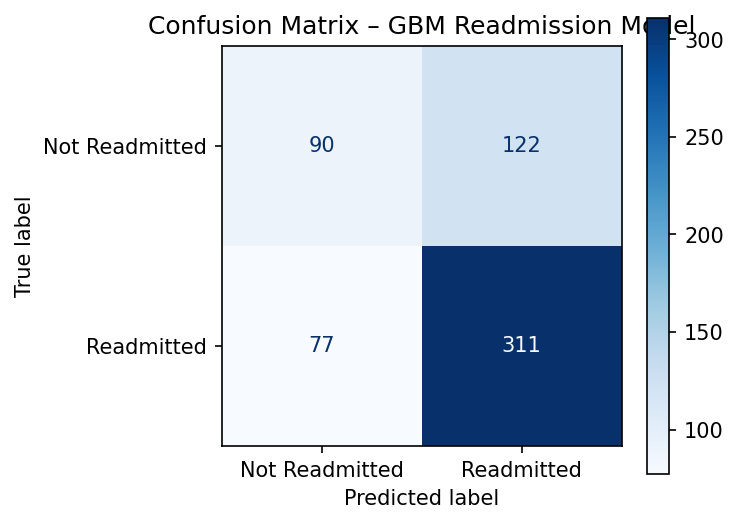
\includegraphics[width=0.55\textwidth]{confusion_matrix.png}
\caption{\textit{Confusion Matrix for the Baseline Gradient Boosting Classifier.}
Rows represent actual class labels; columns represent predicted labels. The model
achieves higher recall (0.80) for the readmitted class than precision (0.72),
reflecting the class imbalance in the dataset.}
\end{figure}

\section{Development of the Explainable AI Solution}

The XAI solution was implemented locally in a Jupyter notebook, mirroring the
``Getting Explanations Locally in Notebook'' workflow described in the Vertex AI
Explainable AI documentation. Integrated Gradients was applied to the MLP
classifier because IG requires a smooth, differentiable model output. The IG
completeness property was verified empirically: the sum of attributions (0.2886)
closely matched $f(x) - f(\text{baseline}) = 0.2892$, confirming correct
implementation. Sampled Shapley was applied to the Gradient Boosting Classifier
via SHAP KernelExplainer, and exact SHAP values were computed using TreeExplainer
as a ground-truth reference.

\begin{figure}[H]
\centering
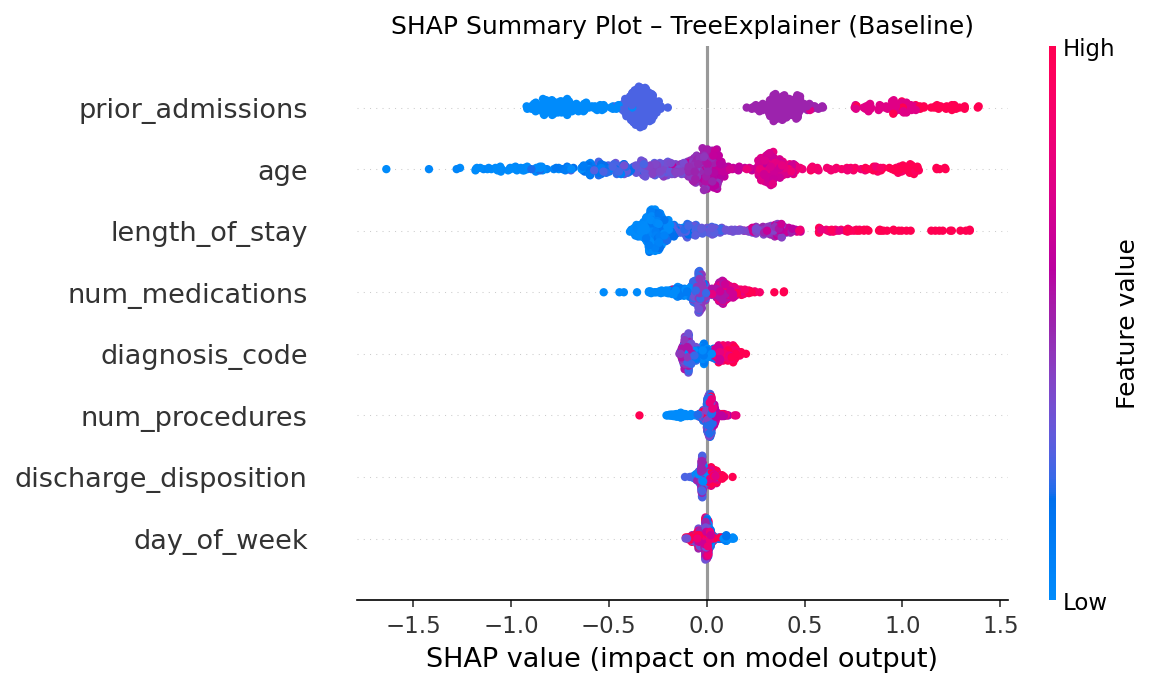
\includegraphics[width=0.85\textwidth]{shap_summary_tree.png}
\caption{\textit{Global SHAP Summary Plot (TreeExplainer, Gradient Boosting Classifier).}
Each dot represents one test instance. Feature importance is ranked by mean
$|$SHAP value$|$. \texttt{prior\_admissions}, \texttt{age}, and
\texttt{length\_of\_stay} are the dominant predictors; \texttt{day\_of\_week}
ranks last, confirming its spurious nature.}
\end{figure}

\subsection{Integrated Gradients: Varying the Number of Steps}

Three step configurations were evaluated: 50, 200, and 500. All three produced
consistent feature rankings---\texttt{prior\_admissions} (attribution $+0.211$),
\texttt{discharge\_disposition} ($+0.093$), and \texttt{num\_medications}
($+0.051$) as the top positive contributors---demonstrating that the MLP had
learned clinically meaningful patterns. The L2 distance between the 50-step and
500-step results was 0.0026, while the 200-step result was already within 0.0014
of the 500-step solution. Inference latency scaled from 0.04~s at 50 steps to
0.11~s at 500 steps---a $2.8\times$ increase---with only marginal attribution
improvement beyond 200 steps. A convergence sweep across nine step counts
confirmed a clear diminishing-return curve with an elbow near 100 steps, making
200 steps the practical optimum for this dataset and model architecture.

\begin{figure}[H]
\centering
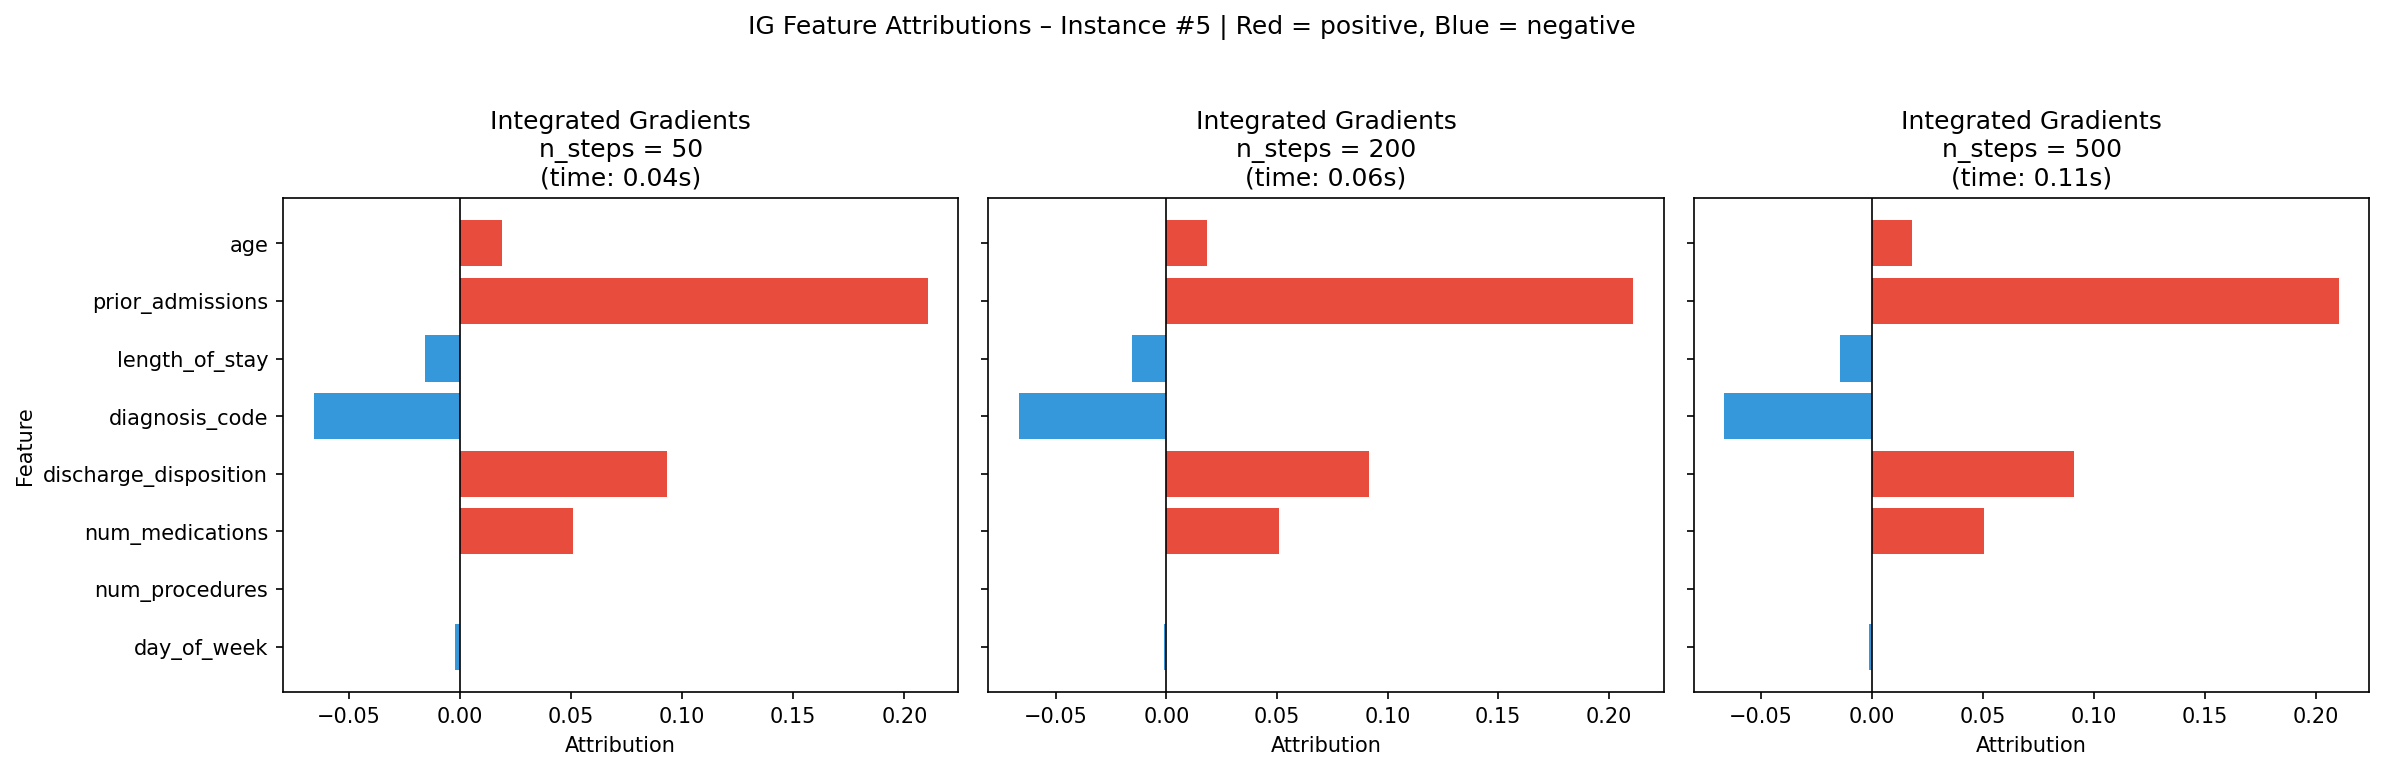
\includegraphics[width=\textwidth]{ig_attributions_comparison.png}
\caption{\textit{Integrated Gradients Feature Attributions Across Step Configurations (MLP).}
Each panel shows per-feature attributions for a single test instance at 50, 200,
and 500 steps. Red bars indicate positive contributions to readmission risk;
blue bars indicate negative contributions. Attribution rankings are stable across
all three configurations.}
\end{figure}

\begin{figure}[H]
\centering
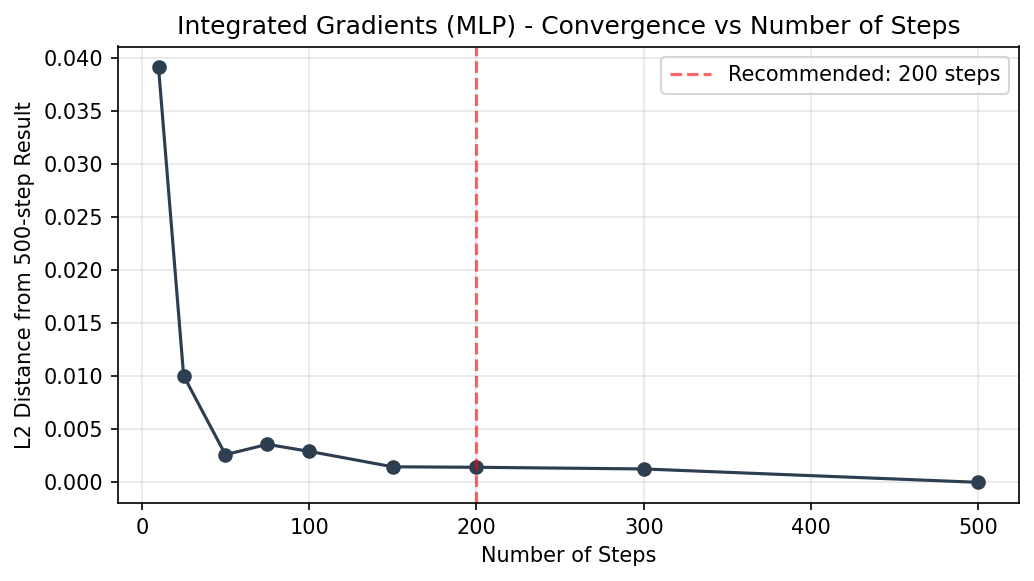
\includegraphics[width=0.75\textwidth]{ig_convergence.png}
\caption{\textit{Integrated Gradients Convergence: L2 Distance from the 500-Step Reference.}
The curve shows rapid convergence up to approximately 100 steps, after which
marginal improvement diminishes substantially. The dashed red line marks the
recommended 200-step configuration.}
\end{figure}

\subsection{Sampled Shapley: Varying the Number of Paths}

A secondary experiment used SHAP KernelExplainer with \texttt{nsamples} of 10,
30, and 50---the direct analogue of the Vertex AI Sampled Shapley
\texttt{num\_paths} parameter (Ribeiro et al., 2016). The L2 distance from the
exact TreeExplainer result was 0.371 at $n = 10$, 0.366 at $n = 30$, and 0.367 at
$n = 50$. The stable L2 error reflected that background dataset size matters as much as
the number of coalitions sampled. Globally, exact
TreeExplainer results confirmed that \texttt{prior\_admissions}
(mean $|\text{SHAP}| = 0.558$), \texttt{age} (0.381), and
\texttt{length\_of\_stay} (0.296) were the three dominant features---consistent
with published clinical literature on readmission risk. Notably,
\texttt{day\_of\_week} received the lowest attribution (0.026, rank 8 of 8), yet
its non-zero value revealed that the model encoded a weekend coding artifact in
the training data---a data quality issue entirely invisible without XAI.

\begin{figure}[H]
\centering
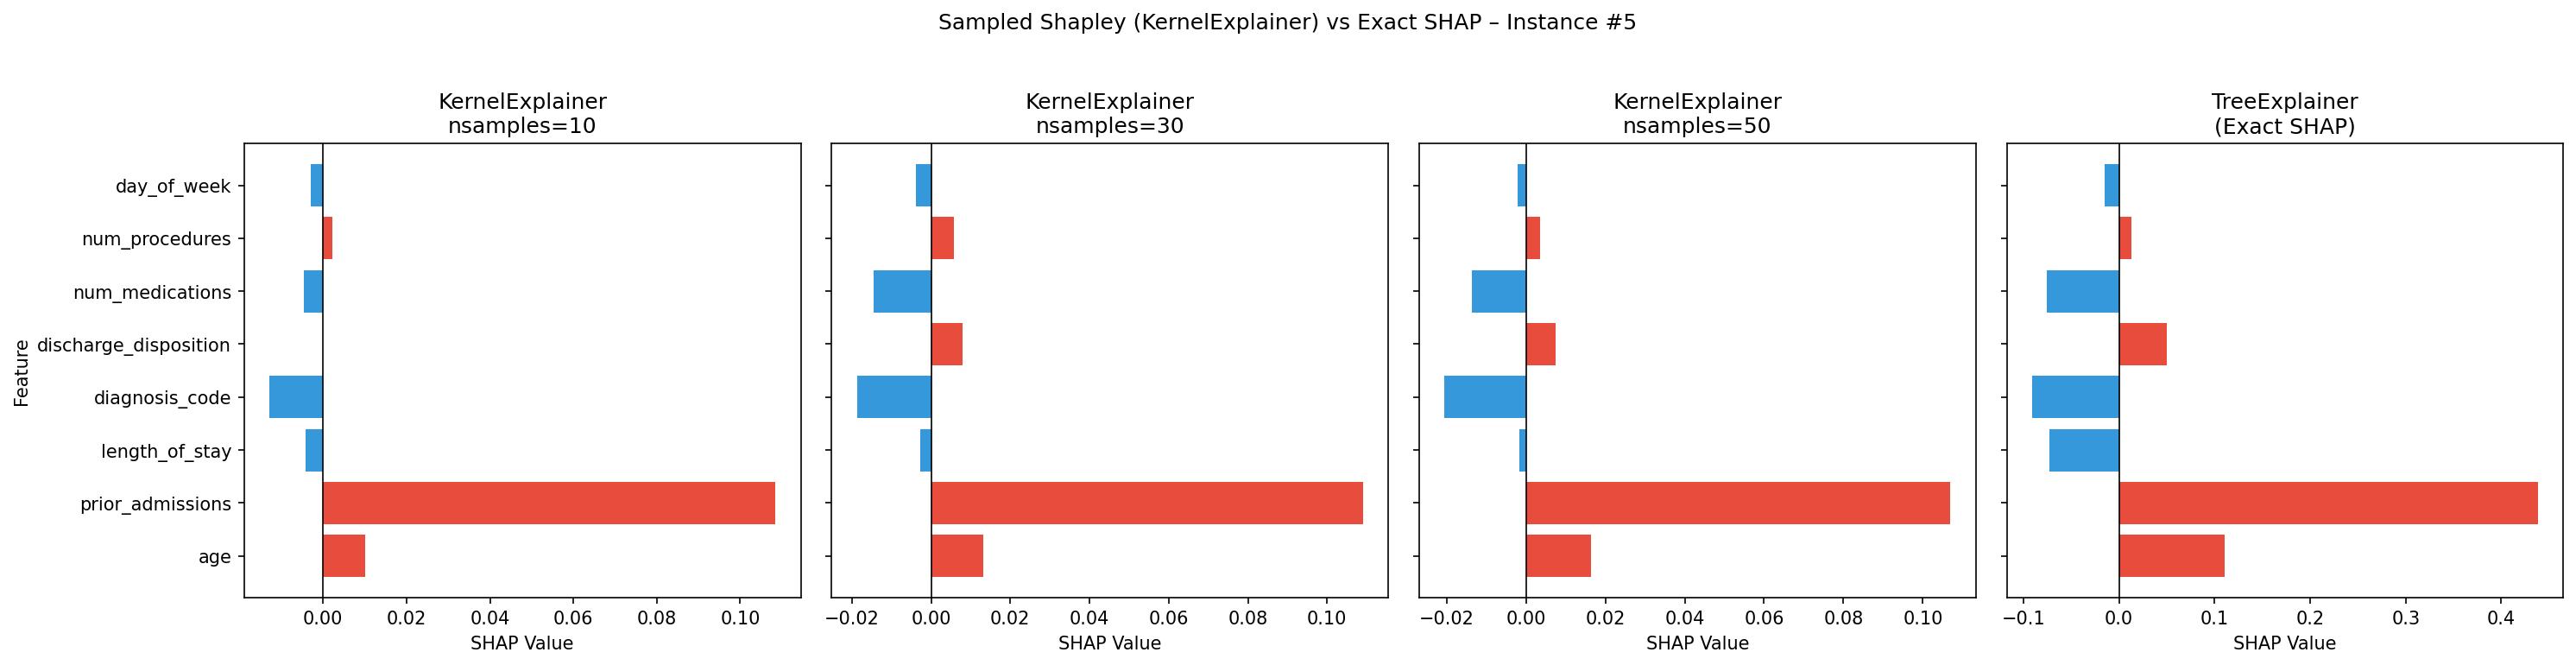
\includegraphics[width=\textwidth]{shap_paths_comparison.png}
\caption{\textit{Sampled Shapley (KernelExplainer) vs.~Exact SHAP (TreeExplainer) Across Path Counts.}
The three left panels show KernelExplainer attributions at nsamples = 10, 30, and
50 for a single test instance. The rightmost panel shows the exact TreeExplainer
values as the reference standard. Attribution direction is consistent across all
configurations; magnitude converges toward the exact values as nsamples increases.}
\end{figure}

\begin{figure}[H]
\centering
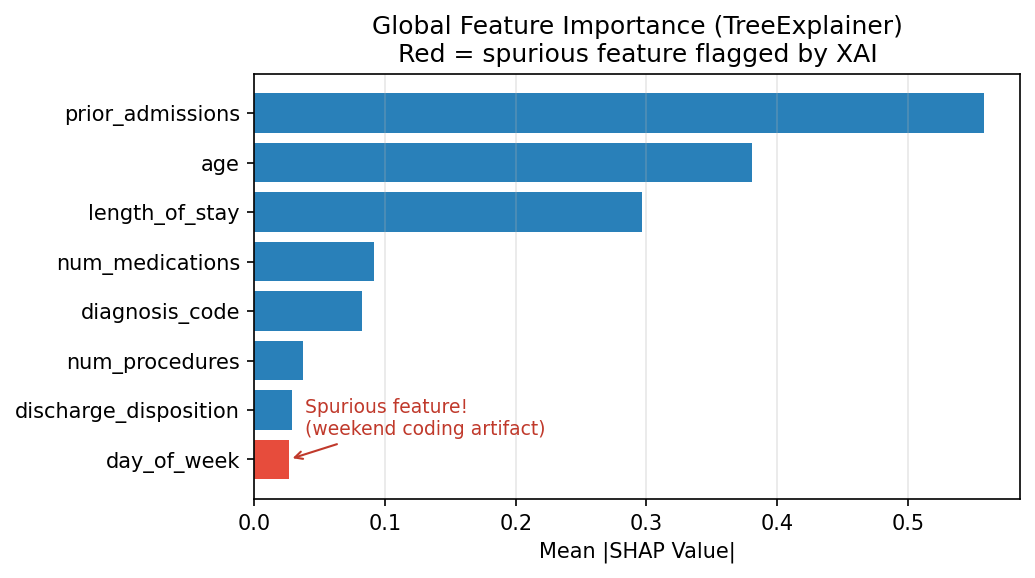
\includegraphics[width=0.75\textwidth]{global_importance_spurious.png}
\caption{\textit{Global Feature Importance with Spurious Feature Highlighted.}
Bars represent mean absolute SHAP values across the test set. The red bar
(\texttt{day\_of\_week}) flags the artifact feature injected into the training
data. Its non-zero global importance confirms the model encoded this spurious
correlation despite it ranking last overall.}
\end{figure}

\section{Lessons Learned and Future Pipeline Implications}

Several important lessons emerged from this exploration, many of which connect
directly to predictive performance outcomes. First, the moderate AUC-ROC of 0.68
achieved by the baseline Gradient Boosting Classifier (improved to 0.69 after grid
search) revealed that the model had limited discriminative power---a performance
ceiling that XAI helped explain rather than conceal. The SHAP attribution analysis showed that \texttt{prior\_admissions}
dominated predictions (mean $|\text{SHAP}| = 0.558$) while several other features
contributed minimally, suggesting that feature engineering---such as admission history interaction
terms---could materially improve predictive performance in future iterations.
XAI did not merely describe the model; it diagnosed it.

Second, the detection of a non-zero attribution for \texttt{day\_of\_week}
demonstrated that the model had learned a spurious correlation from training data,
which would silently degrade generalization on future data where weekend
coding patterns differ. Without XAI, this predictive performance risk
would have been entirely invisible at model evaluation time. This underscores the
need to treat XAI as a diagnostic complement to standard evaluation metrics, not
a substitute.

Third, the comparison between the best GBM (AUC-ROC 0.69) and the MLP (AUC-ROC 0.66)
highlighted a performance-interpretability tradeoff: the MLP was required for
Integrated Gradients due to its smooth output surface, yet it performed slightly
worse. Future pipelines should incorporate both model types in parallel---the
best-performing model for prediction and a differentiable surrogate for
IG-based attribution---so that neither predictive performance nor explanatory
fidelity is sacrificed. Platform vendor lock-in, illustrated by the deprecation
of Vertex Explainable AI, further reinforces the need for open-standard tools
such as SHAP (Lundberg \& Lee, 2017) that remain portable and independent of
provider roadmaps.

% ============================================================
%  REFERENCES
% ============================================================
\newpage

\noindent\textbf{References}

\begingroup
\singlespacing
\setlength{\parindent}{-0.5in}
\setlength{\leftskip}{0.5in}
\setlength{\parskip}{10pt}
\setlength{\emergencystretch}{3em}   % allow extra stretch to avoid overfull boxes

\noindent
Doshi-Velez, F., \& Kim, B. (2017). Towards a rigorous science of interpretable
machine learning. \textit{arXiv preprint arXiv:1702.08608}.
\\\small\url{https://arxiv.org/abs/1702.08608}\normalsize

\noindent
Philip, R.~E. (2019, December 13). Explainability of AI: The challenges and
possible workarounds. \textit{Medium}.\\\small
{\sloppy\url{https://medium.com/@rohithaelsa/explainability-of-ai-the-challenges-and-possible-workarounds-14d8389d2515}\par}\normalsize

\noindent
Google Cloud. (2026a). Get explanations. \textit{Vertex AI documentation}.
\\\small\url{https://docs.cloud.google.com/vertex-ai/docs/explainable-ai/getting-explanations}\normalsize

\noindent
Google Cloud. (2026b). Introduction to Gemini Enterprise Agent Platform pipelines.
\textit{Google Cloud documentation}.
\\\small\url{https://docs.cloud.google.com/gemini-enterprise-agent-platform/machine-learning/pipelines/introduction}\normalsize

\noindent
Lipton, Z.\ C.\ (2018). The mythos of model interpretability.
\textit{Queue, 16}(3), 31--57.
\\\small\url{https://doi.org/10.1145/3236386.3241340}\normalsize

\noindent
Lundberg, S.\ M., \& Lee, S.\ I.\ (2017). A unified approach to interpreting model
predictions. \textit{Advances in Neural Information Processing Systems, 30},
4765--4774.
\\\small\url{https://papers.nips.cc/paper/2017}\normalsize

\noindent
Ribeiro, M.\ T., Singh, S., \& Guestrin, C.\ (2016). ``Why should I trust you?'':
Explaining the predictions of any classifier. \textit{Proceedings of the 22nd ACM
SIGKDD International Conference on Knowledge Discovery and Data Mining},
1135--1144.
\\\small\url{https://doi.org/10.1145/2939672.2939778}\normalsize

\noindent
Sundararajan, M., Taly, A., \& Yan, Q.\ (2017). Axiomatic attribution for deep
networks. \textit{Proceedings of the 34th International Conference on Machine
Learning, 70}, 3319--3328.
\\\small\url{https://proceedings.mlr.press/v70/sundararajan17a.html}\normalsize

\endgroup
\end{document}